\documentclass{article}
\usepackage{amsmath, sfmath, pgfplots, multicol}
\pgfplotsset{compat = newest}
\usepgfplotslibrary{statistics}
\usepackage[margin = 0.5in]{geometry}
\renewcommand{\familydefault}{\sfdefault}
\setlength\parindent{0cm}
\pagestyle{empty}

\newcounter{pset}
\newcounter{key}


\begin{document}

\subsection*{Histograms P-Set}

The body temperatures, in degrees Fahrenheit, of 200 randomly selected hospital patients is shown below.

\begin{center}
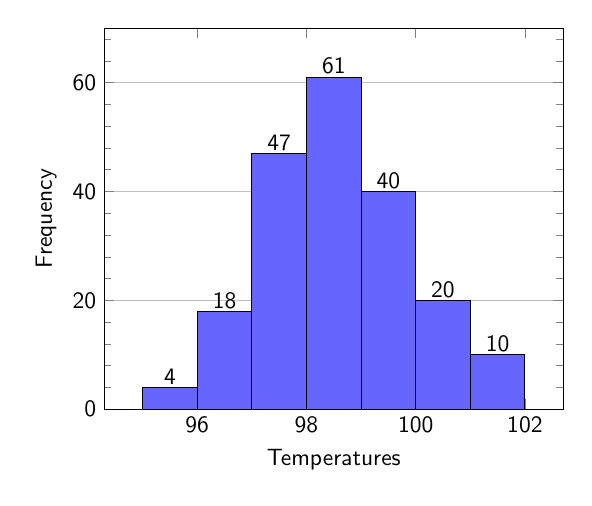
\begin{tikzpicture}[scale=0.85]
\begin{axis}[
ymin = 0, ymax = 70, xlabel = {Temperatures}, ylabel = {Frequency}, ymajorgrids, minor y tick num = 4
]
\addplot[ybar interval, fill=blue!60, mark=no] plot coordinates {(95,4) (96,18) (97,47) (98,61) (99,40) (100,20) (101,10) (102,10)};
\node at (axis cs: 95.5,6) {4};
\node at (axis cs: 96.5,20) {18};
\node at (axis cs: 97.5,49) {47};
\node at (axis cs: 98.5,63) {61};
\node at (axis cs: 99.5,42) {40};
\node at (axis cs: 100.5,22) {20};
\node at (axis cs: 101.5,12) {10};
\end{axis}
\end{tikzpicture}
\end{center}

\begin{enumerate}
    \item How many classes are shown?
    \item What is the class width?
    \item What is the class midpoint of the 3rd class?
    \item What is the lower class limit of the 1st class?
    \item What is the lower class limit of the 4th class?
    \item How many body temperatures are between 98 and 100 degrees?
    \item What is the relative frequency of the 2nd class? Write your answer as a reduced fraction.
    \item What percent of patients have body temperatures between 98 and 100 degrees?
    \item Create a relative frequency histogram for the histogram above.
    \item Create a cumulative frequency histogram for the histogram above.
    \item How many body temperatures are less than 97 degrees?
\end{enumerate}

\newpage 

\texttt{Key}

\begin{enumerate}
    \item 7
    \item 1
    \item 97.5
    \item 95
    \item 98
    \item 101
    \item 9/100
    \item 50.5\%
    \item \mbox{} \newline\\
    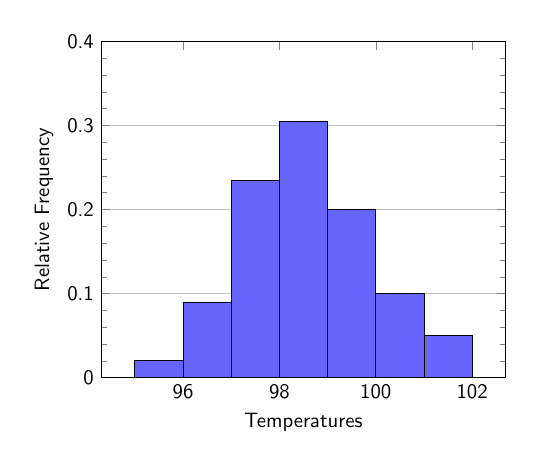
\begin{tikzpicture}[scale=0.75]
    \begin{axis}[
    ymin = 0, ymax = 0.4, xlabel = {Temperatures}, ylabel = {Relative Frequency}, ymajorgrids, minor y tick num = 4
    ]
    \addplot[ybar interval, fill=blue!60, mark=no] plot coordinates {(95,4/200) (96,18/200) (97,47/200) (98,61/200) (99,40/200) (100,20/200) (101,10/200) (102,10/200)};
    \end{axis}
    \end{tikzpicture}
    \item \mbox{} \newline\\
    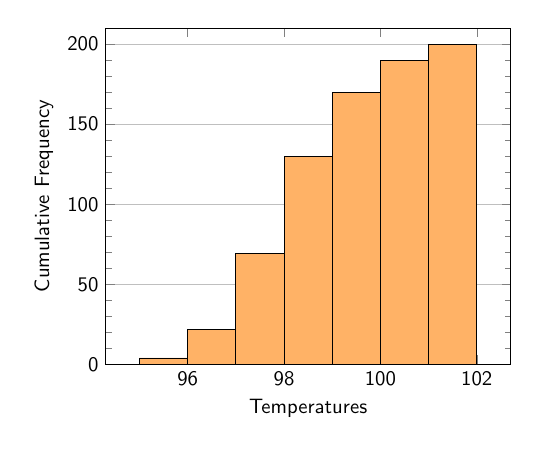
\begin{tikzpicture}[scale=0.75]
    \begin{axis}[
    ymin = 0, ymax = 210, xlabel = {Temperatures}, ylabel = {Cumulative Frequency}, ymajorgrids, minor y tick num = 4
    ]
    \addplot[ybar interval, fill=orange!60, mark=no] plot coordinates {(95,4) (96,22) (97,69) (98,130) (99,170) (100,190) (101,200) (102,200)};
    \end{axis}
    \end{tikzpicture}
    \item 22
\end{enumerate}

\end{document}
